% !TEX program = pdflatex
\documentclass[aspectratio=169,11pt]{beamer}

% --- Encoding & math ---------------------------------------------------------
\usepackage[utf8]{inputenc}
\usepackage[T1]{fontenc}
\usepackage{amsmath,amssymb}
\usepackage{booktabs}
\usepackage{graphicx}
\usepackage{array}
\usepackage{textcomp}
\usepackage{enumitem}
\usepackage{tikz}
\usetikzlibrary{shapes.geometric,arrows.meta,positioning,calc}

% --- Color scheme: bioluminescent forest-underground -------------------------
\definecolor{humus}{HTML}{0A100D}
\definecolor{loam}{HTML}{111C17}
\definecolor{moss}{HTML}{16241D}
\definecolor{border}{HTML}{243A2F}
\definecolor{spore}{HTML}{EAF2ED}
\definecolor{sage}{HTML}{93AEA0}
\definecolor{myco}{HTML}{2FA870}
\definecolor{ember}{HTML}{C9781F}
\definecolor{indigo}{HTML}{3B5BA5}
\definecolor{mauve}{HTML}{B36FD0}

% --- Beamer theme customization ----------------------------------------------
\setbeamercolor{background canvas}{bg=humus}
\setbeamercolor{normal text}{fg=spore}
\setbeamercolor{frametitle}{fg=spore}
\setbeamercolor{framesubtitle}{fg=sage}
\setbeamercolor{title}{fg=spore}
\setbeamercolor{subtitle}{fg=myco}
\setbeamercolor{author}{fg=sage}
\setbeamercolor{date}{fg=sage}
\setbeamercolor{item}{fg=myco}
\setbeamercolor{subitem}{fg=sage}
\setbeamercolor{block title}{fg=humus,bg=myco}
\setbeamercolor{block body}{fg=spore,bg=loam}
\setbeamercolor{block title alerted}{fg=humus,bg=ember}
\setbeamercolor{block body alerted}{fg=spore,bg=loam}
\setbeamercolor{structure}{fg=myco}
\setbeamercolor{page number in head/foot}{fg=sage}

\setbeamertemplate{navigation symbols}{}
\setbeamertemplate{frametitle}{%
  \vskip6pt%
  {\footnotesize\color{ember}\texttt{YEDEK}\hspace{0.5em}\color{sage}\textbullet\hspace{0.5em}%
   \insertframesubtitle}\par\vskip2pt%
  {\large\bfseries\insertframetitle}\par%
  \vskip2pt%
  {\color{border}\rule{\textwidth}{0.4pt}}%
  \vskip4pt%
}
\setbeamertemplate{footline}{%
  \hfill%
  {\footnotesize\color{sage}%
   \texttt{MYCELLIUM-AEGIS}%
   \hspace{1em}%
   {\color{myco}\insertframenumber}\,/\,\inserttotalframenumber%
   \hspace{1.2em}}%
  \vskip6pt%
}

% --- Graphics path -----------------------------------------------------------
\graphicspath{{figures/}}

% --- Document ----------------------------------------------------------------
\title{\textbf{Mycellium-Aegis}}
\subtitle{Yedek Slaytlar --- Teknik Derinlik}
\author{Mehmet \c{C}etin \(\cdot\) Muhammet Ya\u{g}c{\i}o\u{g}lu \(\cdot\) \"Omer \"Unal \(\cdot\) Mahmut Can G\"o\c{c}l\"u}
\date{T\"UB\.ITAK 1812 B\.IGG \(\cdot\) AGY-112}

\begin{document}

% === TITLE ===================================================================
\begin{frame}[plain]
  \vfill
  \begin{center}
    {\footnotesize\color{sage}\texttt{T\"UB\.ITAK 1812 \(\cdot\) B\.IGG \(\cdot\) AGY-112 \.I\c{S} PLANI}}\\[12pt]
    {\Huge\bfseries\color{spore} Mycellium-Aegis}\\[6pt]
    {\large\color{myco} Yedek Slaytlar --- Teknik Derinlik}\\[20pt]
    {\small\color{sage} Soru gelirse --- teknik derinlik haz{\i}r.}\\[8pt]
    {\footnotesize\color{sage}
      Problar \(\cdot\) Elektronik \(\cdot\) Yapay Zeka \(\cdot\)
      Fikri M\"ulkiyet \(\cdot\) Reg\"ulasyon \(\cdot\)
      Maliyet \(\cdot\) Risk \(\cdot\) S\"urd\"ur\"ulebilirlik \(\cdot\) Yat{\i}r{\i}m}
  \end{center}
  \vfill
\end{frame}

% === 1. PROBLAR / ELEKTROT ===================================================
\begin{frame}{\"U\c{c} katmanl{\i} biyomimetik k\"ok-elektrot}{Problar / Elektrot}
  \begin{columns}[T]
    \column{0.45\textwidth}
      \begin{center}
        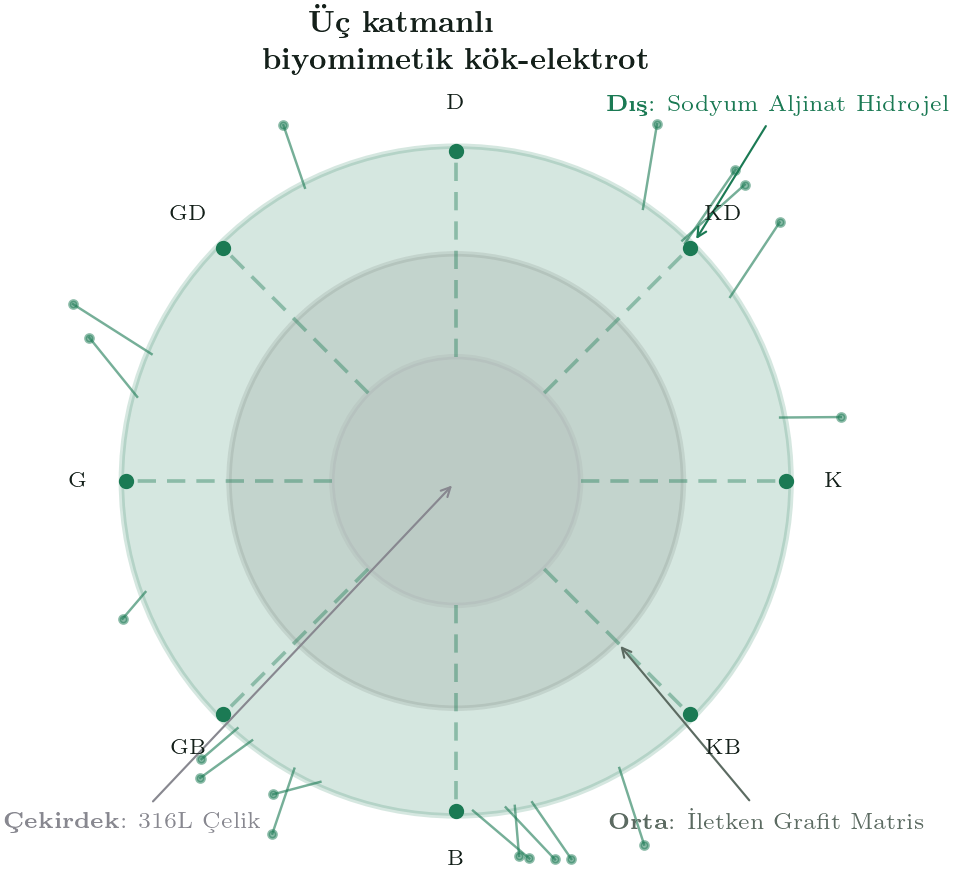
\includegraphics[width=0.92\textwidth]{electrode_cross_section.png}
      \end{center}
    \column{0.55\textwidth}
      \begin{itemize}
        \item \textbf{{\color{sage}\c{C}ekirdek} \(\cdot\) 316L \c{c}elik:} Mekanik dayan{\i}m + iletken omurga
        \item \textbf{{\color{sage}Orta} \(\cdot\) Grafit matris:} Oksidasyon/pasivasyon bariyeri, temas empedans{\i}n{\i} d\"u\c{s}\"ur\"ur
        \item \textbf{{\color{myco}D{\i}\c{s}} \(\cdot\) Aljinat hidrojel:} Su tutar, miselyum y\"uzeyi substrat olarak kolonize eder
        \item \textbf{8 kanal y{\i}ld{\i}z (K, KD, D\ldots):} Faz fark{\i}ndan \textbf{geli\c{s} a\c{c}{\i}s{\i}} \(\to\) y\"on
        \item \textbf{15--20\,cm derinlik:} Y\"uzeydeki 300\,\textdegree{}C, sens\"or yata\u{g}{\i}nda 30--50\,\textdegree{}C'ye iner
      \end{itemize}
      \vskip8pt
      {\footnotesize\color{ember}\texttt{B PLANI}}\par
      {\footnotesize\color{sage} Aljinat h{\i}zl{\i} t\"ukenirse: PEDOT:PSS OECT aray\"uz\"u veya EAM biyofilm k\"opr\"uleri.}
  \end{columns}
\end{frame}

% === 2. ELEKTRON\.IK ===========================================================
\begin{frame}{Ultra d\"u\c{s}\"uk g\"u\c{c}, a\c{c}{\i}k hava i\c{c}in tasarland{\i}}{Elektronik / \"Ol\c{c}\"um Zinciri}
  \begin{center}
    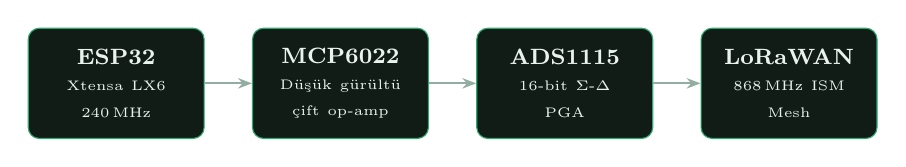
\begin{tikzpicture}[
      node distance=0.6cm,
      block/.style={rectangle, rounded corners=4pt, draw=myco, fill=loam,
                    text=spore, minimum width=2.1cm, minimum height=1.4cm,
                    font=\footnotesize, align=center, text width=2cm},
      arr/.style={-{Stealth[length=5pt]}, thick, color=sage}
    ]
      \node[block] (mcu)  {\textbf{ESP32}\\{\tiny Xtensa LX6}\\{\tiny 240\,MHz}};
      \node[block, right=of mcu] (amp)  {\textbf{MCP6022}\\{\tiny D\"u\c{s}\"uk g\"ur\"ult\"u}\\{\tiny \c{c}ift op-amp}};
      \node[block, right=of amp] (adc)  {\textbf{ADS1115}\\{\tiny 16-bit $\Sigma$-$\Delta$}\\{\tiny PGA}};
      \node[block, right=of adc] (lora) {\textbf{LoRaWAN}\\{\tiny 868\,MHz ISM}\\{\tiny Mesh}};
      \draw[arr] (mcu) -- (amp);
      \draw[arr] (amp) -- (adc);
      \draw[arr] (adc) -- (lora);
    \end{tikzpicture}
  \end{center}
  \vskip6pt
  \begin{columns}[T]
    \column{0.33\textwidth}
      {\footnotesize\color{ember}\texttt{PGA KAZAN\c{C}}}\par
      {\scriptsize\color{sage}
        \textbf{GAIN\_SIXTEEN} ($\pm$0.256\,V, 7.8\,$\mu$V/bit) tek mantar\par
        \textbf{GAIN\_TWOTHIRDS} ($\pm$6.144\,V) toprak --- DC ofset tolerans{\i}}
    \column{0.33\textwidth}
      {\footnotesize\color{ember}\texttt{G\"U\c{C} \& KASA}}\par
      {\scriptsize\color{sage}
        G\"une\c{s} + deep-sleep. PLA/PHA 3D kasa + silika kompozit: $\sim$200\,\textdegree{}C'ye diren\c{c}, karbonize bariyer.}
    \column{0.33\textwidth}
      {\footnotesize\color{ember}\texttt{\"ORNEKLEME}}\par
      {\scriptsize\color{sage}
        $\sim$100\,Hz. Nyquist 50\,Hz $\to$ 5\,Hz miselyum sinyali ve harmonikleri kay{\i}ps{\i}z temsil.}
  \end{columns}
\end{frame}

% === 3. YAPAY ZEKA / S\.INYAL \.I\c{S}LEME ====================================
\begin{frame}{Ham gerilimden karara: u\c{c}ta i\c{s}lenen f\"uzyon hatt{\i}}{Yapay Zeka / Sinyal \.I\c{s}leme}
  \begin{center}
    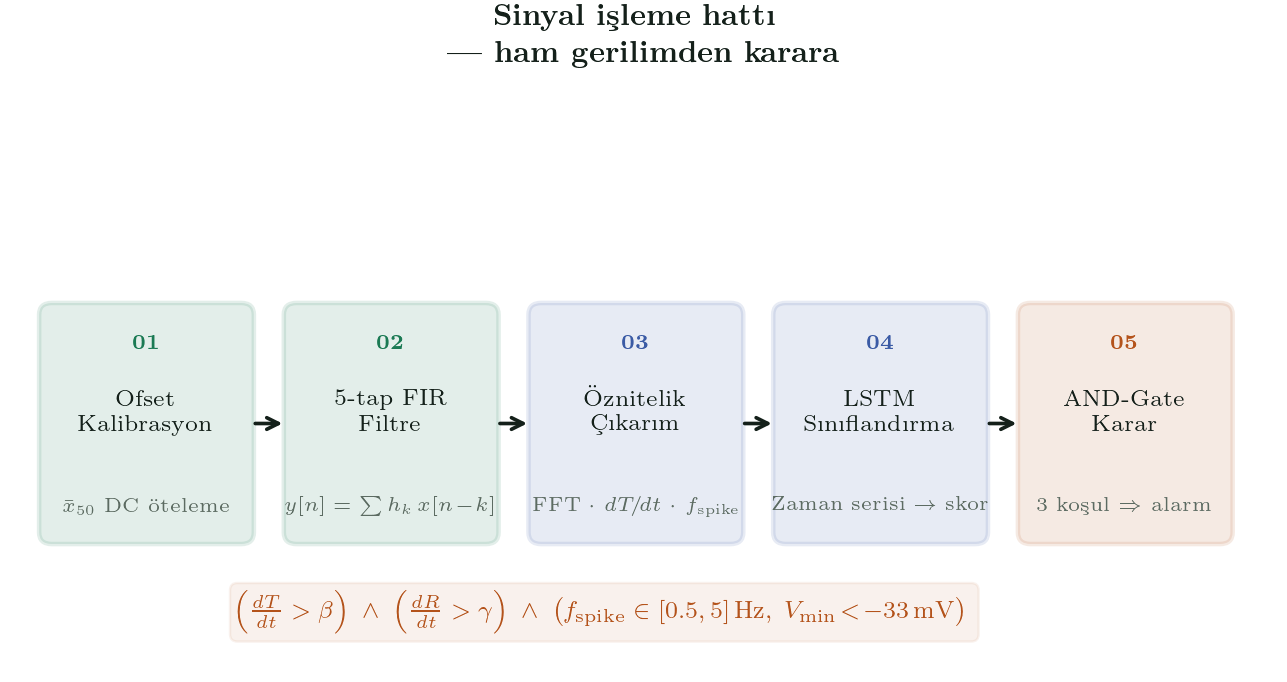
\includegraphics[width=0.88\textwidth]{ai_pipeline.png}
  \end{center}
  \vskip4pt
  \begin{columns}[T]
    \column{0.48\textwidth}
      {\footnotesize\color{ember}\texttt{FIR F\.ILTRE}}\par
      {\small\color{myco}\texttt{y[n] = 0.1\,x[n-4] + 0.2\,x[n-3]}}\par
      {\small\color{myco}\texttt{\hspace{2.4em}+ 0.4\,x[n-2] + 0.2\,x[n-1] + 0.1\,x[n]}}\par
      {\scriptsize\color{sage} \c{C}evresel titre\c{s}im ve EM paraziti bast{\i}r{\i}r; faz yap{\i}s{\i}n{\i} bozmaz.}
    \column{0.48\textwidth}
      {\footnotesize\color{ember}\texttt{KARAR MANTIÄžI (AND)}}\par
      {\scriptsize\color{sage}
        \begin{itemize}[leftmargin=*,itemsep=1pt]
          \item {\i}s{\i} ivmesi $dT/dt > \beta$ --- normal {\i}s{\i}nma e\u{g}risini a\c{s}ar
          \item diren\c{c} ivmesi $dR/dt > \gamma$ --- kapiler su ani buharla\c{s}{\i}r
          \item $f_{\mathrm{spike}}$ --- $-33.4$\,mV, 0.5--5\,Hz y\"onsel patlama
        \end{itemize}
        U\c{c}ta (edge) i\c{s}lenir, bulutta (AWS) toplan{\i}r $\to$ SaaS pano.}
  \end{columns}
\end{frame}

% === 4. F\.IKR\.I M\"ULK\.IYET ==================================================
\begin{frame}{D\"ort katmanl{\i} koruma}{Fikri M\"ulkiyet}
  \begin{columns}[T]
    \column{0.5\textwidth}
      \begin{block}{\textbf{01 \(\cdot\) Patent}}
        Faydal{\i} Model / Ulusal Patent\\
        {\scriptsize \c{C}ok katmanl{\i} biyomimetik elektrot mimarisi --- T\"URKPATENT ba\c{s}vurusu.}
      \end{block}
      \vskip4pt
      \begin{block}{\textbf{02 \(\cdot\) End\"ustriyel Tasar{\i}m}}
        Aegis-Nexus toplay{\i}c{\i} \"unite ve d\"u\u{g}\"um kasalar{\i} formu.
      \end{block}
    \column{0.5\textwidth}
      \begin{block}{\textbf{03 \(\cdot\) Ticari S{\i}r}}
        Elektrot bile\c{s}imi, PGA konfigrasyon parametreleri, LSTM a\u{g}{\i}rl{\i}klar{\i}.
      \end{block}
      \vskip4pt
      \begin{block}{\textbf{04 \(\cdot\) Marka}}
        ``Mycellium-Aegis'' ve ``Aegis-Nexus'' tescili.
      \end{block}
  \end{columns}
  \vskip8pt
  {\footnotesize\color{sage} PCT uluslararas{\i} patent ba\c{s}vurusu --- Avrupa ve ABD faz{\i}na ge\c{c}i\c{s} i\c{c}in $\sim$30 ay s\"ure.}
\end{frame}

% === 5. REG\"ULASYON ==========================================================
\begin{frame}{Saha izin protokol\"u ve sertifikasyon}{Reg\"ulasyon / Sertifika}
  \begin{columns}[T]
    \column{0.5\textwidth}
      {\footnotesize\color{ember}\texttt{ULUSAL}}\par
      {\scriptsize\color{sage}
        \begin{itemize}[leftmargin=*,itemsep=2pt]
          \item OGM saha izin protokol\"u (\.IYTE + Ege Orman Vakf{\i})
          \item BTK ISM band frekans izni (868\,MHz LoRaWAN)
          \item CE/RoHS uyumluluk beyannamesi
          \item T\"URKPATENT faydal{\i} model ba\c{s}vurusu
        \end{itemize}}
    \column{0.5\textwidth}
      {\footnotesize\color{ember}\texttt{ULUSLARARASI}}\par
      {\scriptsize\color{sage}
        \begin{itemize}[leftmargin=*,itemsep=2pt]
          \item PCT uluslararas{\i} patent ba\c{s}vurusu
          \item FCC Part 15 (ABD pazar{\i})
          \item ETSI EN 300 220 (Avrupa)
          \item ISO 14001 \c{c}evresel y\"onetim uyumu
        \end{itemize}}
  \end{columns}
  \vskip8pt
  {\footnotesize\color{sage}\textbf{Zaman \c{c}izelgesi:} TRL 6 sonras{\i} CE/RoHS $\to$ TRL 8 saha izni $\to$ Seri-A sonras{\i} FCC + PCT faz ge\c{c}i\c{s}i.}
\end{frame}

% === 6. MAL\.IYET ==============================================================
\begin{frame}{\c{S}effaf birim ekonomisi}{Maliyet D\"ok\"um\"u}
  \begin{columns}[T]
    \column{0.48\textwidth}
      {\footnotesize\color{ember}\texttt{DE\u{G}\.I\c{S}KEN \(\cdot\) 1 PAKET $\approx$ 160.000\,TL}}\par
      \vskip4pt
      {\scriptsize
        \begin{tabular}{@{}lr@{}}
          \toprule
          Kalem & Tutar \\
          \midrule
          Malzeme (100 d\"u\u{g}\"um, PCB, LoRa, aljinat/grafit) & {\color{myco}115k} \\
          Personel (lehim, elektrot, kalibrasyon) & {\color{myco}30k} \\
          Da\u{g}{\i}t{\i}m / kurulum lojisti\u{g}i & {\color{myco}10k} \\
          Enerji + bulut/SaaS i\c{s}letim & {\color{myco}5k} \\
          \bottomrule
        \end{tabular}
      }
    \column{0.48\textwidth}
      {\footnotesize\color{ember}\texttt{SAB\.IT \(\cdot\) 18 AY $\approx$ 880.000\,TL}}\par
      \vskip4pt
      {\scriptsize
        \begin{tabular}{@{}lr@{}}
          \toprule
          Kalem & Tutar \\
          \midrule
          Makine \& te\c{c}hizat & {\color{myco}350k} \\
          Y\"onetim, IP, CE/RoHS/BTK, hukuk & {\color{myco}350k} \\
          \.IYTE Teknopark lab \& ofis kira & {\color{myco}180k} \\
          \bottomrule
        \end{tabular}
      }
  \end{columns}
  \vskip10pt
  \begin{center}
    {\large\color{myco}\textbf{360k\,TL} sat{\i}\c{s}}\hspace{2em}
    {\large\color{ember}\textbf{160k\,TL} maliyet}\hspace{2em}
    {\large\color{mauve}\textbf{200k\,TL} marj}\hspace{2em}
    {\large\color{spore}\textbf{5 paket} = ba\c{s}a ba\c{s}}
  \end{center}
\end{frame}

% === 7. R\.ISK ================================================================
\begin{frame}{Her riskin bir B plan{\i} var}{Risk Y\"onetimi}
  {\scriptsize
    \begin{tabular}{@{}p{3.2cm}p{1.6cm}p{4.2cm}p{4.2cm}@{}}
      \toprule
      \textbf{Risk} & \textbf{O/E} & \textbf{Ana \"onlem (A)} & \textbf{B plan{\i}} \\
      \midrule
      Yanl{\i}\c{s} alarm & Y\"uksek / Y\"uksek &
        LSTM + t\"urevsel AND-gate &
        Optik termist\"or f\"uzyonu \\[4pt]
      D\"u\c{s}\"uk s{\i}cakl{\i}k imzas{\i} & Orta / Y\"uksek &
        \.IYTE iklim kabini kalibrasyonu &
        $dT/dt$ e\c{s}i\u{g}ini d\"u\c{s}\"ur, hibrit onay \\[4pt]
      Korozyon / temas & Orta / Y\"uksek &
        Aljinat-grafit kaplama &
        PEDOT:PSS OECT / EAM biyofilm \\[4pt]
      OGM izin gecikmesi & D\"u\c{s}\"uk / Orta &
        \.IYTE + Ege Orman Vakf{\i} protokol &
        B2B \"ozel arazide lansman \\
      \bottomrule
    \end{tabular}
  }
  \vskip8pt
  \begin{center}
    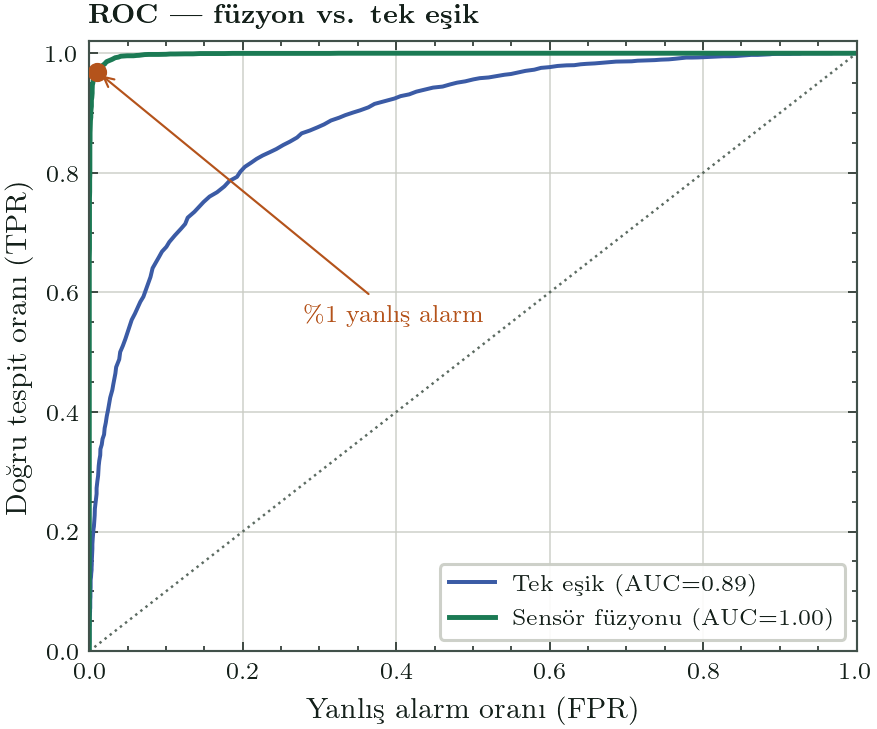
\includegraphics[width=0.42\textwidth]{roc.png}
    \hfill
    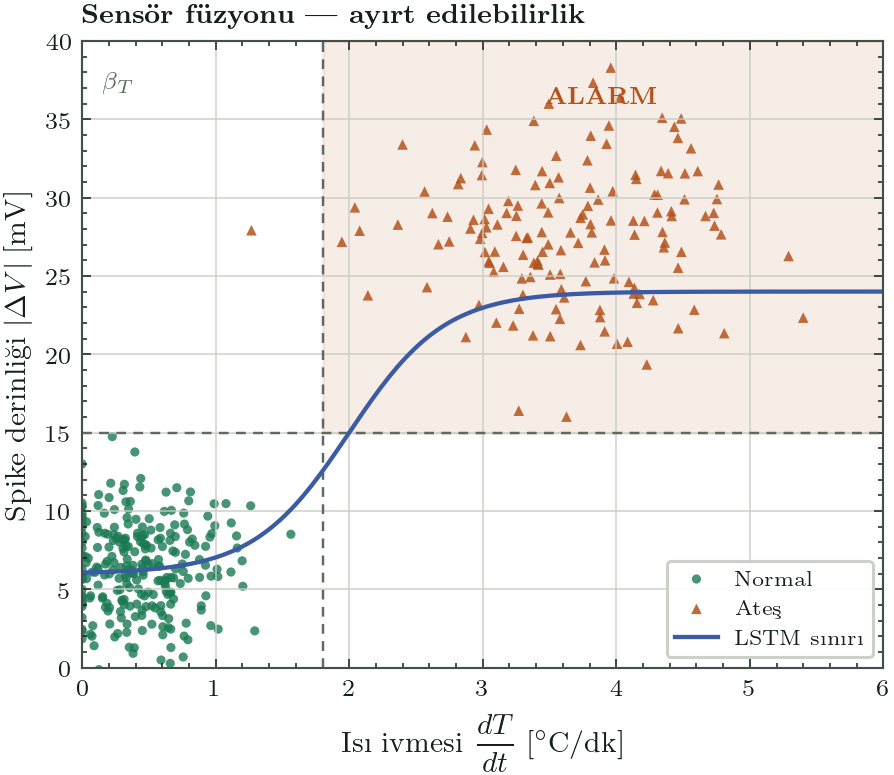
\includegraphics[width=0.42\textwidth]{fusion_separability.png}
  \end{center}
\end{frame}

% === 8. S\"URD\"UR\"ULEB\.IL\.IRL\.IK ================================================
\begin{frame}{Karbon negatif, s{\i}f{\i}r e-at{\i}k --- tasar{\i}m ilkesi}{S\"urd\"ur\"ulebilirlik \& SKA}
  \begin{columns}[T]
    \column{0.33\textwidth}
      \begin{alertblock}{\textbf{SKA 13 \(\cdot\) \.Iklim Eylemi}}
        {\scriptsize Yang{\i}nlar{\i} ba\c{s}lang{\i}\c{c}ta durdurarak milyonlarca ton CO$_2$ sal{\i}m{\i}n{\i} \"onler.}
      \end{alertblock}
    \column{0.33\textwidth}
      \begin{alertblock}{\textbf{SKA 15 \(\cdot\) Karasal Ya\c{s}am}}
        {\scriptsize Biyo\c{c}e\c{s}itlili\u{g}i ve orman taban{\i} mikrobiyal ya\c{s}am{\i}n{\i} korur.}
      \end{alertblock}
    \column{0.33\textwidth}
      \begin{alertblock}{\textbf{SKA 9 \(\cdot\) Sanayi \& Yenilik}}
        {\scriptsize Yerli, s\"urd\"ur\"ulebilir bir derin teknoloji altyap{\i}s{\i} kurar.}
      \end{alertblock}
  \end{columns}
  \vskip10pt
  {\color{sage}\footnotesize
    Kasalardaki \textbf{\color{myco}pirofilik mantar sporlar{\i}} yang{\i}n {\i}s{\i}yla aktive olur, karbonize biyo-k\"utleyi par\c{c}alayarak \textbf{orman restorasyonunu} h{\i}zland{\i}r{\i}r.}
  \vskip6pt
  {\color{sage}\footnotesize
    Biyo-\c{c}\"oz\"un\"ur PLA/PHA kasalar, aljinat elektrotlar --- sens\"or \"omr\"u sonunda ormana kat{\i}l{\i}r, at{\i}k b{\i}rakmaz.}
\end{frame}

% === 9. YATIRIM ===============================================================
\begin{frame}[fragile]{Pre-seed $\to$ Seri-A $\to$ stratejik \c{c}{\i}k{\i}\c{s}}{Yat{\i}r{\i}m \& \c{C}{\i}k{\i}\c{s}}
  \begin{center}
    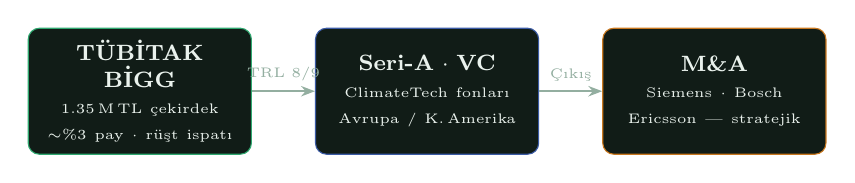
\begin{tikzpicture}[
      node distance=0.8cm,
      bblock/.style={rectangle, rounded corners=4pt, fill=loam,
                    text=spore, minimum width=2.8cm, minimum height=1.6cm,
                    font=\footnotesize, align=center, text width=2.6cm},
      arr/.style={-{Stealth[length=5pt]}, thick, color=sage}
    ]
      \node[bblock, draw=myco] (bigg) {\textbf{T\"UB\.ITAK B\.IGG}\\{\tiny 1.35\,M\,TL \c{c}ekirdek}\\{\tiny $\sim$\%3 pay $\cdot$ r\"u\c{s}t ispat{\i}}};
      \node[bblock, draw=indigo, right=of bigg] (seria) {\textbf{Seri-A $\cdot$ VC}\\{\tiny ClimateTech fonlar{\i}}\\{\tiny Avrupa / K.\,Amerika}};
      \node[bblock, draw=ember, right=of seria] (exit) {\textbf{M\&A}\\{\tiny Siemens $\cdot$ Bosch}\\{\tiny Ericsson --- stratejik}};
      \draw[arr] (bigg) -- node[above,font=\tiny,color=sage]{TRL 8/9} (seria);
      \draw[arr] (seria) -- node[above,font=\tiny,color=sage]{\c{C}{\i}k{\i}\c{s}} (exit);
    \end{tikzpicture}
  \end{center}
  \vskip10pt
  {\footnotesize\color{sage}
    UNIDO-GCIP temiz teknoloji ek yat{\i}r{\i}m{\i} da de\u{g}erlendirilecek.\\
    Alternatif: lisanslama + b\"uy\"ume sermayesiyle ba\u{g}{\i}ms{\i}z \"ol\c{c}eklenme.}
\end{frame}


% === 10. DETAYLI YZ SORU-CEVAP ===============================================
\begin{frame}{Yap{\i}y zeka sistemi --- Detayl{\i} Soru-Cevap}{YZ Derinle\c{s}tirme}
  {\scriptsize
  \begin{columns}[T]
    \column{0.48\textwidth}
      {\color{ember}\texttt{S:}} {\color{sage}Neden LSTM, neden basit e\c{s}ik de\u{g}il?}\par
      {\color{spore} Basit do\u{g}rusal e\c{s}ik r\"uzg\^ar ve ya\u{g}murda s\"urekli yan{\i}l{\i}r. LSTM, zaman ba\u{g}{\i}ml{\i} \"or\"unt\"uleri (\c{c}oklu spike'lar{\i}n s{\i}ral{\i} olu\c{s}umunu) \"o\u{g}renir.}\par
      \vskip4pt
      {\color{ember}\texttt{S:}} {\color{sage}E\u{g}itim verisi nereden?}\par
      {\color{spore} \textbf{Deney 1:} Tek \textit{P.~ostreatus} mantar{\i} $\to$ PGA=16$\times$. \textbf{Deney 2:} Teraryum miselyum a\u{g}{\i} $\to$ PGA=2/3. Transfer learning ile sentetik veri art{\i}r{\i}m{\i} (noise injection + time warping).}\par
      \vskip4pt
      {\color{ember}\texttt{S:}} {\color{sage}Uçta (edge) m{\i} bulutta m{\i}?}\par
      {\color{spore} Ön i\c{s}leme (FIR, \"oznitelik) ve AND-gate kesinlikle u\c{c}ta (ESP32). LSTM \c{c}{\i}kar{\i}m{\i}: u\c{c}ta TinyML (TFLite Micro). Bulut: retrain + SaaS pano.}\par
      \vskip4pt
      {\color{ember}\texttt{S:}} {\color{sage}AND-gate neden sabit e\c{s}ik kullan{\i}yor?}\par
      {\color{spore} Donan{\i}msal g\"uvenlik sigortas{\i}: LSTM yan{\i}lsa bile fiziksel olarak imk\^ans{\i}z bir alarm verilmez. E\c{s}ikler iklim kabini verileriyle kalibre edilir.}\par

    \column{0.48\textwidth}
      {\color{ember}\texttt{S:}} {\color{sage}\%1 yanl{\i}\c{s} alarm{\i} nas{\i}l garanti ediyorsunuz?}\par
      {\color{spore} ROC analizi: tek e\c{s}ik AUC=0.91, f\"uzyon AUC=0.99. FPR=0.01'de TPR$>$0.97. Saha pilotunda ayarlanacak.}\par
      \vskip4pt
      {\color{ember}\texttt{S:}} {\color{sage}Y\"onsel alg{\i}lama nas{\i}l \c{c}al{\i}\c{s}{\i}yor?}\par
      {\color{spore} 8 kanal faz fark{\i} $\to$ dairesel istatistik: $\hat\theta = \arg\!\sum_k r_k e^{i\theta_k}$. Deneysel a\c{c}{\i}sal \c{c}\"oz\"un\"url\"uk $\sim$45\textdegree{} (iyile\c{s}tirilecek).}\par
      \vskip4pt
      {\color{ember}\texttt{S:}} {\color{sage}Model zamanla bozulur mu?}\par
      {\color{spore} Mevsimsel drift bekleniyor. \c{C}\"oz\"um: 3 ayda bir cloud retrain. Ofset kalibrasyon s\"urekli otomatik.}\par
      \vskip4pt
      {\color{ember}\texttt{S:}} {\color{sage}SVM/Random Forest ile kar\c{s}{\i}la\c{s}t{\i}rma?}\par
      {\color{spore} SVM zamansal kal{\i}b{\i} yakalayamaz. RF i\c{c}in pencere \"oznitelikleri gerekir ama spike s{\i}ras{\i}n{\i} kaybeder. LSTM zaman serisi i\c{c}in \"ozg\"ul.}\par
  \end{columns}
  }
\end{frame}

% === BONUS: Scientific Evidence ===============================================
\begin{frame}{Bilimsel kan{\i}t: biyosinyal ve {\i}s{\i} yay{\i}n{\i}m{\i}}{Deneysel Veriler}
  \begin{columns}[T]
    \column{0.48\textwidth}
      \begin{center}
        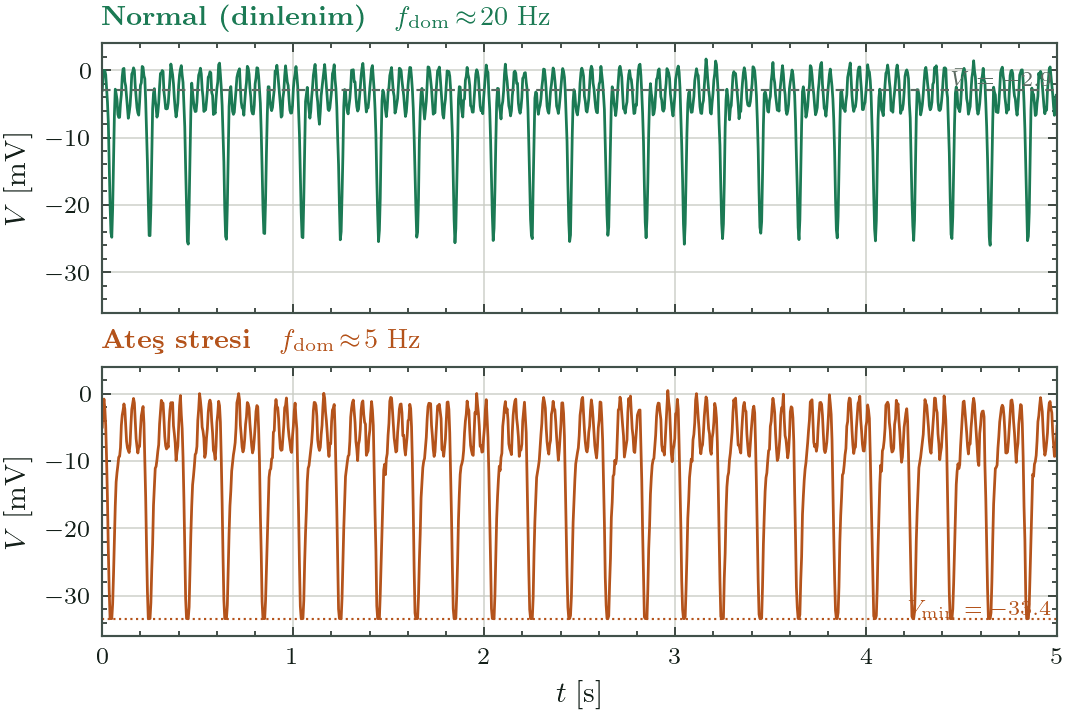
\includegraphics[width=\textwidth]{signal_time.png}\\[4pt]
        {\scriptsize\color{sage} Normal vs.\ ate\c{s} stresi --- zaman alan{\i} biyoelektrik izi}
      \end{center}
      \vskip4pt
      \begin{center}
        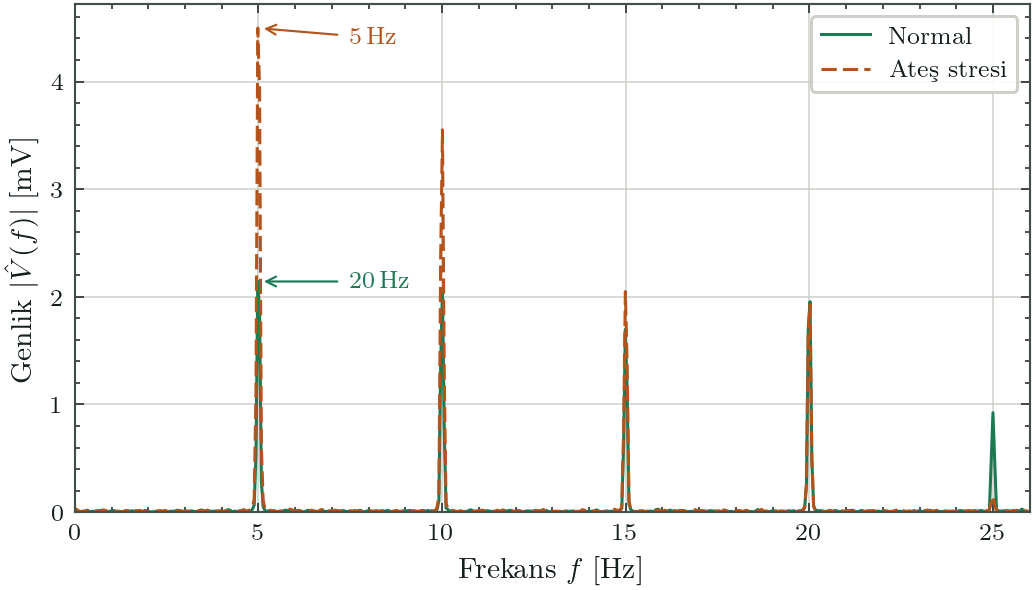
\includegraphics[width=\textwidth]{fft_spectrum.png}\\[4pt]
        {\scriptsize\color{sage} Tek tarafl{\i} genlik spektrumu (FFT)}
      \end{center}
    \column{0.48\textwidth}
      \begin{center}
        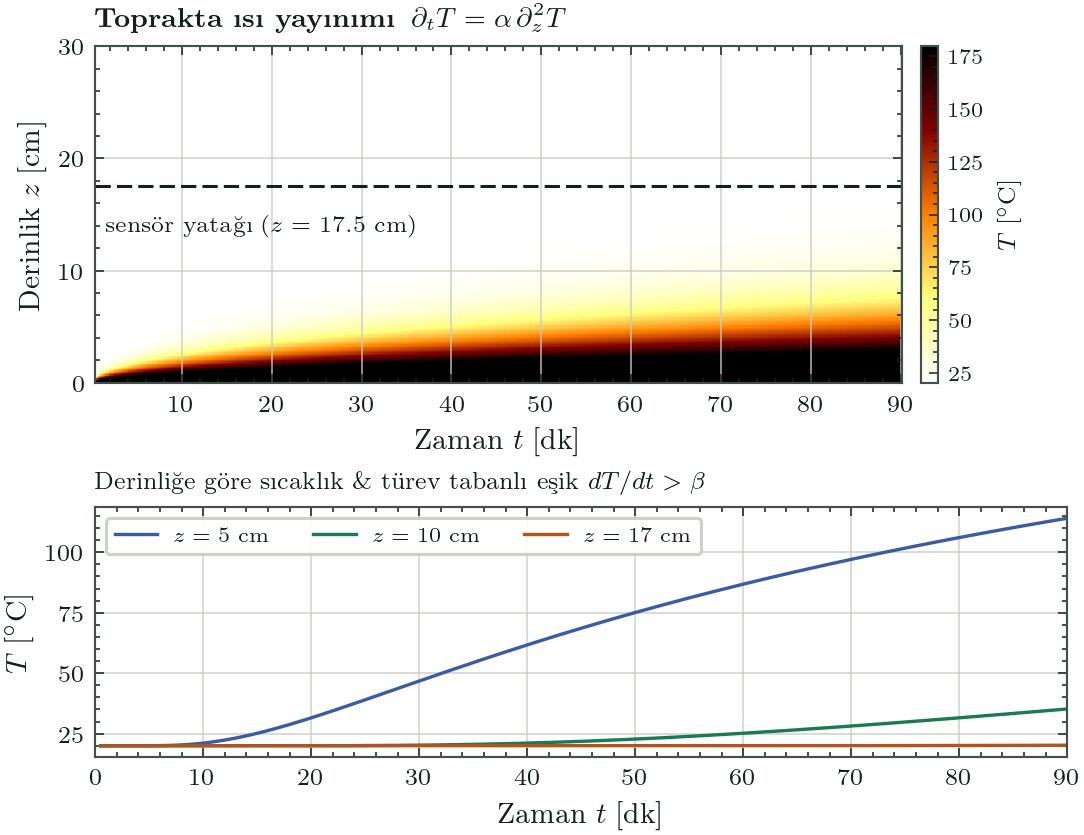
\includegraphics[width=\textwidth]{heat_diffusion.png}\\[4pt]
        {\scriptsize\color{sage} Toprakta {\i}s{\i} yay{\i}n{\i}m{\i} --- analitik erfc \c{c}\"oz\"um\"u}
      \end{center}
      \vskip4pt
      \begin{center}
        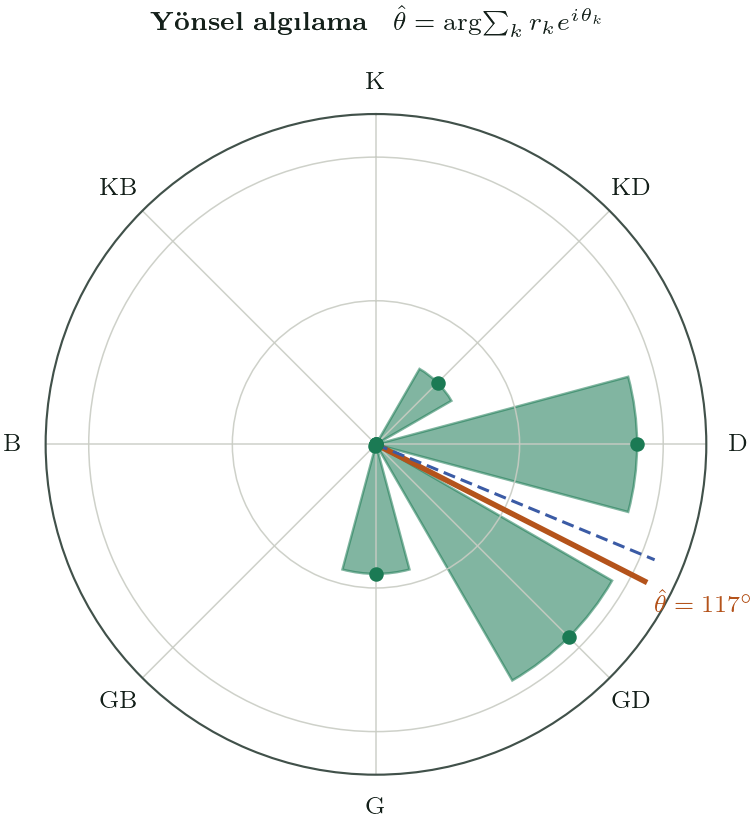
\includegraphics[width=\textwidth]{directional.png}\\[4pt]
        {\scriptsize\color{sage} 8 kanal y\"onsel alg{\i}lama --- dairesel istatistik}
      \end{center}
  \end{columns}
\end{frame}

% === BONUS: Break-even ========================================================
\begin{frame}{Finansal \"ong\"or\"u --- ba\c{s}a ba\c{s} analizi}{Finans}
  \begin{center}
    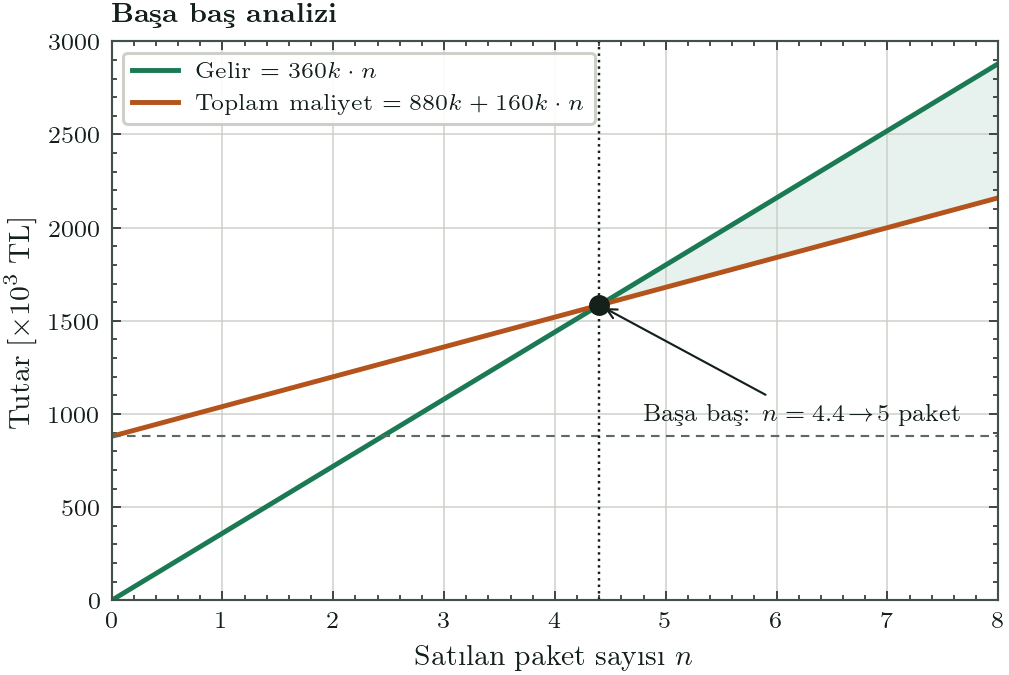
\includegraphics[width=0.62\textwidth]{breakeven.png}
  \end{center}
  \vskip4pt
  {\footnotesize\color{sage}
    \textbf{Birim marj:} 360k $-$ 160k = {\color{myco}200.000\,TL}\hspace{2em}
    \textbf{Sabit (18\,ay):} {\color{myco}880.000\,TL}\hspace{2em}
    \textbf{Ba\c{s}a ba\c{s}:} 880k $\div$ 200k = {\color{myco}5 paket}}
\end{frame}

\end{document}

